\chapter{Data}
\label{Chapter2}
\lhead{Chapter 2. \emph{Data}}

In this chapter, I discuss the data, surveys and the follow-up facilities used in this thesis. I begin by discussing the Supernova Legacy Survey (SNLS) which was used in the early parts of this thesis and was the source of data for my work on the rate of SLSNe at z$\sim$1, discussed in \cref{Chapter3}. Following from this, I discuss the Dark Energy Survey (DES) which provided a larger and higher redshift sample of transients used in my search for high redshift SLSNe as described in \cref{Chapter5}. I outline the spectroscopically confirmed sample of SLSN used as the ground truth sample for comparison to the sample presented in \cref{Chapter6}. I also give an overview of the SUDSS survey, which provided some auxiliary data for the DES SLSN sample. Throughout the chapter, I briefly describe the follow-up facilities used in the classifying of SLSNe that were discovered in real time during the operation of SNLS as well as the SN that were targeted using the selection techniques discussed in \cref{Chapter5} as part of DES. Finally, I describe the process of collecting and unifying the sample of published SLSNe used as a baseline training dataset throughout this work.

\section{Supernova Legacy Survey}
The Supernova Legacy Survey \citep{Boulade2003,Pritchet2004} was run as part of the Canadian-French-Hawaii Telescope Legacy Survey (CFHT-LS) between 2003 and 2008. Over that time, it was proven to be one of the most successful SN surveys to date, observing thousands of transients and spectroscopically confirming a large proportion of them. This included over 300 SN-Ia \citep{Perrett2010} and more than 50 core-collapse supernovae as well as measuring their respective rates \citep{Perrett2012,Bazin2009}. SNLS has also discovered two SLSNe at $z$=1.588 and $z$=1.50 \citep{Howell2013} which, until recently, have been the highest redshift spectroscopically identified objects of this class. The principal objective of the survey was to perform a measurement of the cosmological constants $\omega_{\Lambda}$ and $\omega_{m}$ \citep{Astier2006}. This was extremely successful, producing the most precise ground-based measurement of its time \citep{Sullivan2006}. This was in large possible thanks to the observing strategy optimized to maximize the number of high redshifts SN-Ia candidates and the thorough spectroscopic follow-up program, which gave much stronger constraints for the Hubble diagram thanks to the high redshift leverage not possible before with the low redshift SN-Ia surveys.

\subsection{Survey Overview}
SNLS used the 4m Canadian-French-Hawaiian Telescope (CFHT) situated on Mauna Kea, Hawaii. It was operated by teams from Canada and France as part of the CFHT Legacy Survey that composed of a small area, deep SN survey and a shallow, wide galaxy survey aimed at studying the large-scale structure of the Universe and the cosmological parameters through galaxy clustering and weak lensing \citep{Pritchet2004,Astier2006}. Four deep fields of $\sim$1 deg$^2$ have been observed to the limiting magnitude of $m\sim$23.5 using the 400-megapixel MegaCam camera \citep{Boulade2003}. Observations took place over five seasons, each lasting approximately 5 months. In total, 202 nights have been allocated to the survey \citep{Pritchet2004}.

\subsection{Cadence and Observations}
SNLS carried out the observations in the \textit{griz} photometric bands, similar in bandpass to the filters used in SDSS \fref{fig:SNLSFilters}. Each field was observed over five to seven periods, each lasting approximately 18 days during the lunar dark times, with an average cadence of 3-4 days \citep{Astier2006,Guy2010}. Where the weather conditions allowed for it, all bands were observed simultaneously on the same night. As a survey aimed at producing a densely populated, high quality and high redshift Hubble diagram, the cadence was optimized to maximize the number of detections of SN-Ia at mid to high redshift (0.2 $\leq$ z $\leq$ 0.9) with a sufficient data quality to perform light curve model fitting \citep{Pritchet2004}. The quality criteria required the light curves to have two detections before and two after the maximum light of the SN, which the cadence used by SNLS was well suited for. In cases where the observing plan could not be fully executed, due to weather condition or otherwise, the \textit{r} and \textit{i} band observations have been prioritized over the \textit{g} and \textit{z} band observations \citep{Guy2010}. This meant that even during the more chaotic, early stages of the survey or suboptimal weather conditions, the quality of the light curves remained good enough for SN-Ia analysis. However, this had a large effect on the \textit{g}-band data in the later stages of the season where the data is often missing due to a shorted observing window where the field was visible. This had an effect on the analysis of the much bluer, in comparison to SN-Ia, SLSN in the sample \citep{Prajs2016}.

\begin{figure}
  \centering
  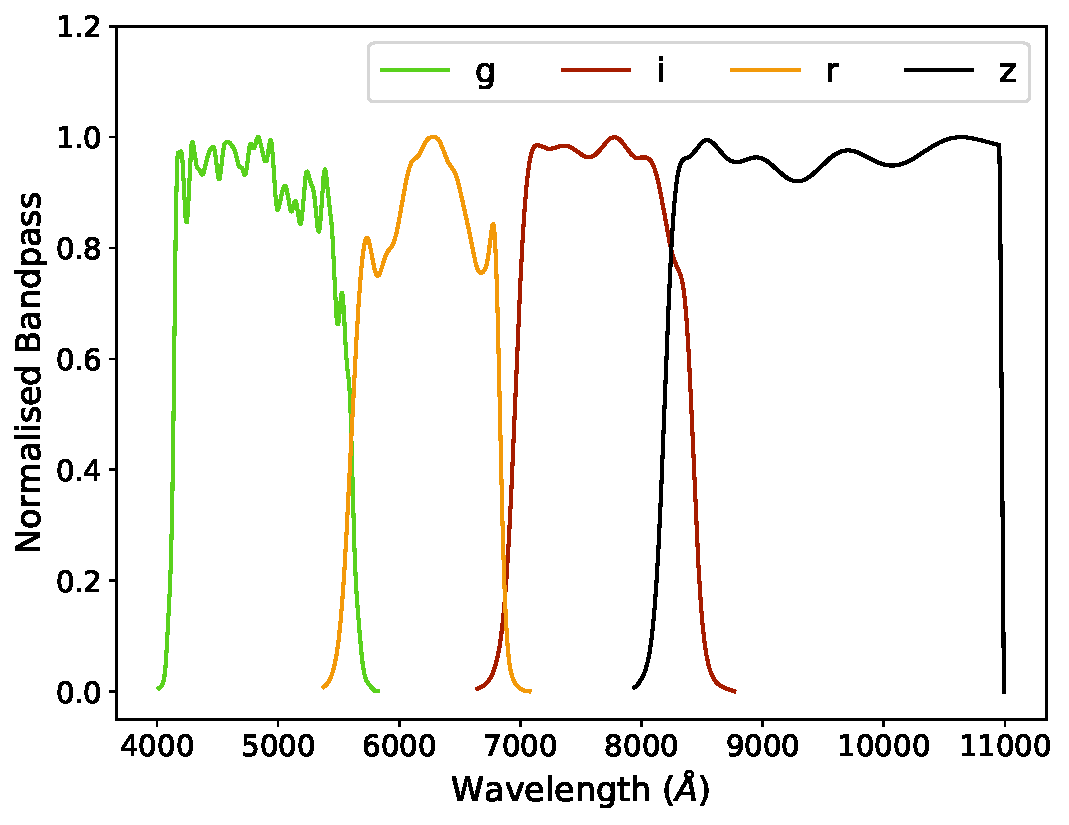
\includegraphics[scale=0.8]{Figures/Chapter2/SNLS_filters.pdf}
    \caption{Bandpass response for filters used in SNLS compared to a spectrum of a SLSN; SNLS06D4eu at z=1.588 discovered by the survey [TODO - PLOT AND BIN IT UP]}
    \label{fig:SNLSFilters}
\end{figure}

\subsection{Data Reduction}
Several different data reduction pipelines have been used in the analysis of the SNLS data. In this thesis, we used a combination of data prepared for public and internal data releases, we have also reanalysis the data for some objects of interest using PTFPhot, a custom, a pre-existing pipeline designed to improve the data reduction quality for faint sources \citep{Firth2015}.

\subsubsection{Real-time photometry}
During the live operations of the survey, the data was pre-processed by applying flats and biases using the \textsc{Elixir} pipeline \citep{Magnier2004}. The data has then been independently analysed by the French and Canadian teams using separate quick-reduction pipelines \citep{Astier2006,Bazin2011}. Both teams aimed to produce lists of new, viable SN candidates within hours of their observations before sending them to the spectroscopic follow-up facilities. Both teams were very successful and produced mostly identical lists which lead to high classification accuracy, largely contributing to the overall success of the survey \citep{Pritchet2004}.

\subsubsection{Forced photometry}
The quick reduction pipelines used in the detection of objects were optimized with speed, as opposed to accuracy, in mind. Any scientific analysis of the data requires a more precise treatment of the photometry. The data for 'real' transient, defined as having detections on multiple epochs and in multiple bands, was passed through an early version of PTFPhot \citep{Firth2015}, a much improved, custom, forced photometry pipeline. The improvements in the photometry, compared to the quick photometry, come mainly from the treatment of the PSF of the images. The quality of the science images is measured precisely on a number of stars, allowing for the reference images, usually with better quality, to be downgraded to match the quality of the science frames by convolving them with the PSF. Furthermore, the photometry is measured at the centroid for the source determined in a stack of all images as opposed to individual frames, giving rise to the term 'forced' photometry as the positions of the objects are forced to be consistent between all images. The full treatment of the PSF largely decreases the uncertainties associated with the flux measurement, especially for faint sources close to, or below, the detection limit. This analysis has been applied to the data releases that provided the sources and light curves for the work described in \cref{Chapter3} in a similar way to other SNLS analysis such as the rates of SN-Ia \citep{Perrett2012} and core-collapse SN \citep{Bazin2009}, as well as the cosmological measurements \citep{Astier2006,Sullivan2011}.

\subsection{Spectroscopic Follow-Up}
The success of SNLS cannot be attributed only to the number of transients discovered by the survey, but also to the effort behind the spectroscopic follow-up of the candidates. Between the Very Large Telescope (VLT), Keck, Gemini North and South and Magellan, more time has been allocated for spectroscopic follow-up than the time allocated to the photometric survey alone \citep{Pritchet2004}. As a result, 322 SN-Ia have been spectroscopically confirmed along with 51 CCSN and two SLSNe \citep{Guy2010,Howell2005,Howell2013}. A large number of the SN confirmed by the survey have been classified before or at their maximum thanks to both the follow-up selection criteria, which correctly identified the most promising candidates \citep{Sullivan2006}, and the readiness of the survey to sacrifice the classification rate in order to improve the quality of the data. While a large number of CCSN and AGN have been targeted for follow-up, which perhaps in the eyes of the primary goal of SNLS could be considered as undesired contaminants, this process also leads to the accidental discovery of two high redshift SLSN. These objects would be almost certainly overlooked if they were targeted post-peak as their evolution would have strongly disfavored them as SN-Ia candidates. In turn, the rapid follow-up of SNLS06D4eu has produced a spectrum at a rest-frame phase of -34 days, which remains to this day as one of the earliest spectra of a SLSN.

\subsection{Redshift measurements}
Distance measurements are invaluable in any type of SN analysis beyond just their application in cosmology. SNLS has provided three types of redshift measurements, used as distance probes: SN spectroscopic redshift, host galaxy spectroscopic redshift and photometric redshift estimates. The case of the SN spectroscopic redshift is the most accurate and rarely disputable as lines used to identify the redshift can be confirmed in the raw spectrographic images to be coincidental with the trace of the SN light. In SNLS this was measured for all classified SN. Furthermore, it may sometimes be possible to measure the redshift of an object that has an ambiguous classification as some spectral features may be strong enough to be detectable despite low S\/N of the continuum.

Similarly to the SN spectroscopy, the host spectroscopy can provide a very high accuracy measurement of the redshift using narrow spectral features. However, it is possible that the host of the object may be misidentified. For example, the redshift might be measured for a bright galaxy apparently coincidental with the SN while the true host was a background galaxy or a dwarf foreground galaxy. Since these errors are relatively rare, we use both the target and host spectroscopic redshifts as absolute. SNLS, similarly to other large SN surveys, was not able to target all potential SN candidates during the live operations of the survey with many unclassified objects, later photometrically selected as good SN candidates after they faded below the detection limit. \citet{Lidman2012} used the AAOmega multi-fibre spectrograph on the Anglo-Australian Telescope (AAT) to target nearly 700 hosts of SN candidates in two of the four SNLS fields, obtaining redshift for 400 of them.

Beyond the spectroscopic measurement, it is also possible to estimate the redshift using the photometry of the galaxies. The SED of a galaxy usually contains a characteristic sharp break at $\sim$4000\AA which can be observed to transition between filters as a function of redshift. This is a very powerful technique which, when used with a number of photometric filters, can very accurately estimate the redshift of a galaxy for $z$>0.3. Below that threshold, the SED break is contained within a single filter largely increasing the uncertainty of the estimate \citep{Connolly1995}. This technique has been used to estimate redshifts for over 500,000 galaxies within the CFHTLS, which overlapped with the SNLS fields giving a redshift estimate to nearly all candidates with a detected host \citep{Ilbert2006}.

\subsection{SLSN in SNLS}
As a survey designed with a heavy focus on SN-Ia, SNLS was not an ideal for detecting SLSN or other transients with relatively peculiar evolution. Its small area and relatively dense cadence meant that the volume searched was not sufficient to the detect a large number of SLSN, known to be a very rare class of astronomical events \citep{Cooke2012,Prajs2016,Quimby2013}. It is therefore perhaps not a coincidence that the only two objects detected by the survey were found at $z$=1.50 and $z$=1.588 where the survey was searching a much greater volume.

Beyond the nominal, live survey, the images for individual SNLS seasons have been co-added together to create "super" stacks, reaching a detection magnitude of $m$=26.5 \citep{Cooke2012}. A further two SLSN candidates have been detected using this technique. Their light curve behaviours were similar to that of a SLSN in terms of the absolute luminosity and temporal evolution. While it was impossible at that point (several years after the explosion time of the SN) to spectroscopically identify these objects, host galaxy spectroscopy was obtained for both objects determining redshifts of $z$=2.05 and $z$=3.9 \citep{Cooke2012}, confirming that these transients had luminosities comparable to that of SLSN. While these candidate SLSNe shows an interesting precedent for what may be hiding beyond the reach of our current 4m telescope class optical surveys, they were not used in any projects within this thesis. The lack of certain confirmation, low cadence in the stacked images light curve and the difference in the detection technique used deemed these objects incompatible with other SLSN data sources \citep{Prajs2016}.

\section{Dark Energy Survey}
The Dark Energy Survey (DES) is the largest cosmology survey operated to date. It is composed of two elements; a wide galaxy survey and a SN component. Its main aim is to perform the most precise to date measurement of the cosmological parameters. Many features and components of DES have been borrowed and improved on from previous surveys including SDSS and SNLS.

\subsection{Survey Setup}
DES uses a purpose build, 570 mega-pixel DECam CCD camera \citep{Honscheid2008,Flaugher2015} mounted on the 4m Blanco telescope at the Cerro-Tollolo observatory in Chile. One of the greatest advantages of DECam over its predecessors is its high sensitivity at red wavelengths allowing for the high signal to noise observations in \textit{z} and \textit{y} bands compared to other surveys and allowing for SN detections at high redshift [INSERT FILTER PLOT]. DES was awarded 500 observing nights over the period of 5 years between 2013 and 2018 \citep{DES2016}. While the SN component has come to an end at the end of the fifth season as originally planned, the DES wide field component has been awarded more time to make up for the time lost due to unusually bad weather conditions in Chile over the last few years. Each season of observations started in late August and continued through to the end of January giving an average length of 5 months.

\subsubsection{Wide Survey}
DES wide survey has been designed to observe 5000 deg$^2$ of the southern sky to the depth of m$\sim$25 in the \textit{ugrizy} filters. The aim of this is to create the largest catalogue of galaxies and their associated redshifts to date at an unprecedented resolution and depth for a ground-based survey, with the first public data release contained a catalogue of 400 million galaxies from the initial 3 years of the survey \citep{DES2018}. These data can be used to study cosmology via three separate experiments; the Baryon Acoustic Oscillations (BYO), Galaxy Clustering and Weak Lensing \citep{DES2016,Prat2017,Drlica-Wagner2017,DES2017}.

\subsubsection{Supernova Survey}
The goal of the DES SN search is to produce the largest, homogeneous catalogue of SN-Ia to date. To achieve this, 10 observing fields have been selected are observed in the \textit{griz} photometric bands. Eight of these fields are 'shallow' and observe to the depth of m=23.5 while two fields have been chosen to be 'deep' and observe to m=25. The number of deep and shallow fields was chosen such as to maximize the number of discovered SN-Ia while still allowing for a sufficient number of high redshift objects to be detected \citep{Bernstein2012}.

\subsubsection{The cadence of the DES}
DES is composed of multiple elements, all with different core scientific and cadence requirements. In order to provide a fair and unbiased data set an automated scheduling algorithm has been used to maximize the scientific output [NEED TO FIND CITATION]. The Weak Lensing experiment provides the strongest constraint to the scheduling process. As it requires the measurement of the shape and orientation of galaxies with maximum available precision, it forces the wide fields to be observed only in the best, sub 1'' seeing conditions. As nights with suboptimal observing conditions are not ideal for the wide survey, the SN fields are observed instead often leading to a relatively dense cadence of low-quality images in cases of persistent bad weather. This is most common at the start of every season when the observation takes place in Chilean Winter/Spring. As the weather improves towards the Summer months, the seeing is rarely bad enough to give preference to the SN fields. To prevent the cadence from becoming too long the field are observed on a "dead man" trigger after 7 nights without observations, regardless of the conditions.

\subsection{Data Reduction}
While the basic structure and principles behind the data reduction in DES are very similar to that of SNLS, the major differences lay in the treatment of transient detection in the difference images. As the volume of data in DES was too large to allow for manual selection of real sources as a long-term solution. A manual classification was performed only in the first year of the survey operation. This dataset was then used as a training sample for machine learning classification pipeline, \textsc{autoScan} \cite{Goldstein2015}.

Thanks to a large number of computing resources available to the survey the computationally expensive force photometry have been automatically performed on every transient candidate, defines as an object with at least three detections in a minimum of two different bands where the detections were within 30 days but not all on the same night.

Further to Force Photometry, DES has recently developed a Scene Modeling Photometry (SMP) pipeline for use with the SN data. SMP can greatly reduce the uncertainties associated with transient photometry by removing the requirement for template images. Instead of subtracting a template that was downgraded in quality from science frames, the pixels in the region surrounding a transient are modelled individually as constant values with a variable source placed over them. The models are then processed to match the quality of the images before they are ingested into a fitting routine. While this technique provides data with the superior quality it was introduced into the survey at a very late stage of this thesis making it impossible to be implemented.

\subsection{Spectroscopic redshift}
One of the biggest differences in the design of DES versus other SNIa surveys is its approach to redshift measurements.

\subsubsection{Host galaxy redshift}
From the predicted number of objects to be detected by DES, it was clear, since the early planning stages, that it would be impossible to obtain spectroscopic redshift using the SN spectra for all the candidates. The survey, therefore, focused on obtaining the spectroscopic redshift of the host galaxy for all objects. This is being achieved in collaboration with OzDES, an Australian survey using the AAOmega multi-fibre spectrograph mounted on the AAT telescope dedicated to spectroscopic follow-up of DES SN fields. All real transients are targeted regardless of the brightness of their host as the target is observed multiple times over the duration of the survey and the spectra are stacked. Is some cases redshift has been measured in galaxies down to 24.5 magnitudes. Furthermore, DES SN fields were purposely selected to overlap with other surveys in order to provide a catalogue of redshifts for galaxies in the fields. This included Chandra Deep Field South (CDF-S), European Large Area ISO Survey (ELAIS), XMM Large Scale Structure survey (XMM-LSS) as well as SNLS and the SDSS Stripe82 regions.

\subsubsection{Hostless SN}
<<<<<<< HEAD
While redshifts for the majority of SNe can be obtained from their hosts, there remain some that are associated with galaxies fainter than the detection limit of even the stacked AAT spectra. For these objects, it is critical that the redshifts are measured during the live transient which has been the main focus of the extensive spectroscopic campaign. A number of facilities including VLT, Keck, Magellan, MMT, SALT SOAR and NTT amongst others have been used, giving a total of XXX hours or observing time. xxx SNIa have been classified along with xx CCSN and xx SLSNe. A short description and circumstances involving the classification of DES SLSN are described in \sref{sec: DES_SLSN} [ASK MAT FOR CHRIS'S PAPER TO FIX THESE]
=======
While redshifts for the majority of SNe can be obtained from their hosts, there remain some that are associated with galaxies fainter than the detection limit of even the stacked AAT spectra. For these objects, it is critical that the redshifts are measured during the live transient which has been the main focus of the extensive spectroscopic campaign. A number of facilities including VLT, Keck, Magellan, MMT, SALT SOAR and NTT amongst others have been used, giving a total of XXX hours or observing time. xxx SNIa has been classified along with xx CCSN and xx SLSNe. A short description and circumstances involving the classification of DES SLSN are described in \sref{sec:DES_SLSN} [ASK MAT FOR CHRIS'S PAPER TO FIX THESE]
>>>>>>> 41086f048c5b1eec2643a48889278c8c6627c784

\subsection{Photometric Redshifts}
All experiments that form part of DES rely heavily on photometric redshift measurements making it an integral part of the survey. The wide component uses the measurement as a base for their cosmological measurements as it is currently impossible to measure spectroscopic redshifts for even a fraction of the nearly half a billion galaxies detected by DES. The SN survey used the measurements as redshift priors in transient classification. These fits are not used for cosmology, instead, they act as a prioritizing tool for the spectroscopic follow-up program. Photometric redshifts have also been used as part of the SLSN search. While most SLSNe would be expected to have a faint or no host associated with them thanks to their common association with dwarf galaxies, we have used the photometric information (also the lack of it) as a possible sign that an object may be a SLSN, e.g. in cases where the galaxy was measured to be too local or where there was no photometric redshift present meaning that the object can be considered as 'hostless'. This is described in more details in \cref{Chapter5}.

\subsection{SLSNe in DES}
\label{sec:DES_SLSN}
While SLSNe have never been a primary target of DES, their potential use as cosmological probes \citep{Inserra2014} meant that they have generated a large interest within the survey. The first SLSN, and the only one detected in the first season of the survey, DES13S2cmm has been classified using a Directors Discretionary Time (DTT) program at the VLT and was published as one of the earliest results from DES \cite{Papadopoulos2015}. In the following seasons, the number of objects discovered has increased dramatically with $\sim$6 objects confirmed per year, giving motivation to the photometric search for the missing SLSN in the data performed in this thesis. The sample (Angus et al. in prep), has shown a large diversity of the objects with many falling outside of the 'classical' definition of a SLSN \citep{Inserra2018}. I briefly outline the spectroscopic sample from the first four years of DES and its interesting properties as well as any peculiarities in the light curve or spectral evolution in the context of their modelling and comparisons with the photometric sample of SLSN described in \cref{Chapter6}. The sample is summarized in \tref{tab:desSLSN}

\begin{table}
\begin{center}
    \caption{Summary of the DES spectroscopic sample of SLSNe.}
    \label{tab:desSLSN}
\begin{tabular}{|l|r|l|l|l|l|}
\hline
    \multicolumn{1}{|c|}{Name} &
    \multicolumn{1}{c|}{Redshift} &
    \multicolumn{1}{c|}{Peak M$_u$} &
    \multicolumn{1}{c|}{RA} &
    \multicolumn{1}{c|}{DEC} &
    \multicolumn{1}{c|}{Reference} \\

\hline
    DES13S2cmm  &   0.663  &    -19.9  &    02:42:32.83    &    -01:21:30.1 & \citet{Papadopoulos2015}\\
\hline
    DES14C1fi   &   1.4    &    -21.9  &    03:33:49.80    &    -27:03:31.6 & Angus et al. (in Prep.)\\
    DES14C1rhg  &   0.481  &    -19.2  &    03:38:07.27    &    -27:42:45.7 & Angus et al. (in Prep.)\\
    DES14E2slp  &   0.57   &    -20.5  &    00:33:04.08    &    -44:11:42.8 & Angus et al. (in Prep.)\\
    DES14S2qri  &   1.5    &    -21.6  &    02:43:32.14    &    -01:07:34.2 & Angus et al. (in Prep.)\\
    DES14X2byo  &   0.869  &    -21.6  &    02:23:46.93    &    -06:08:12.3 & Angus et al. (in Prep.)\\
    DES14X3taz  &   0.608  &    -21.6  &    02:28:04.46    &    -04:05:12.7 & \citet{Smith2016}\\
\hline
    DES15C3hav  &   0.39   &    -19.1  &    03:31:52.17    &    -28:15:09.5 & Angus et al. (in Prep.)\\
    DES15E2mlf  &   1.86   &    -22.1  &    00:41:33.40    &    -43:27:17.2 &  \citet{Pan2017}\\
    DES15S1nog  &   0.565  &    -20.0  &    02:52:14.98    &    -00:44:36.3 & Angus et al. (in Prep.)\\
    DES15S2nr   &   0.22   &    -20.0  &    02:40:44.62    &    -00:53:26.4 & Angus et al. (in Prep.)\\
    DES15X1noe  &   1.188  &    -22.5  &    02:14:41.93    &    -04:52:54.5 & Angus et al. (in Prep.)\\
    DES15X3hm   &   0.86   &    -21.8  &    02:26:54.96    &    -05:03:38.0 & Angus et al. (in Prep.)\\
\hline
    DES16C2aix  &   1.07   &    -20.6  &    03:40:41.17    &    -29:22:48.4 & Angus et al. (in Prep.)\\
    DES16C2nm   &   1.998  &    -22.3  &    03:40:14.83    &    -29:05:53.5 & \citet{Smith2018}\\
    DES16C3cv   &   0.727  &    -20.7  &    03:40:14.83    &    -29:05:53.5 & Angus et al. (in Prep.)\\
    DES16C3dmp  &   0.526  &    -20.5  &    03:31:28.35    &    -28:32:28.3 & Angus et al. (in Prep.)\\
    DES16C3ggu  &   0.95   &    -21.4  &    03:31:12.00    &    -28:34:38.7 & Angus et al. (in Prep.)\\
\hline
\end{tabular}
\end{center}
\end{table}

[MARK: SHOULD THIS SECTION HAVE PLOTS OF ALL SLSNE FOUND IN DES OR SHOULD I PUT THIS IN THE APPENDIX]

\subsubsection{DES13S2cmm}
DES13S2cmm was the first SLSN discovered by DES. It was identified during a visual light curve scan and quickly selected as a potential SLSN candidate due to its particularly long rise and faint host. A spectrum of the SN has been obtained with the VLT/FORS2 using a DDT program. The observation confirmed that the SN is at z=0.609 and has features comparable to a SLSNe. At the time of discovery, this was one of the lowest luminosities SLSNe at M$_u$=-19.9.

\subsubsection{DES14C1fi}
DES14C1fi was similarly identified as a plausible candidate using a manual search thanks to its slow evolution. It was observed at the Keck telescope and again, 7 days later, using VLT/XShooter which found a featureless continuum that was a very good match to a blackbody SED. A 3728\AA oxygen emission doublet was used to identify the redshift as z=1.30 giving it a luminosity of M$_u$ = -21.9. While this result is somewhat tentative due to a very low S\/N in the IR arm of XShooter there is a possible sign of a broad H-alpha feature. DES14C1fi is the only SLSN in the DES sample that shows potential signs of being a SLSN-II candidate in the first four seasons.

\subsubsection{DES14C1rhg}
DES14C1rhg was targeted as a hostless SLSN candidate based on its long rise time of 30 days. It was observed using our VLT/XShooter SLSN program and confirmed at z=0.47 putting it at a lower than expected redshift for a SLSN of that apparent magnitude and giving it a luminosity of M$_u$ = -19.2. Combining its low brightness with a relatively fast decline time puts DES14C1rhg on the extreme of the population making it incompatible with any current photometric definition of a SLSN despite its spectroscopic resemblance. DES14C1rhg gave us the first indication that the DES sample is able to identify objects in the gap between SLSN and SNIc.

\subsubsection{DES14E2slp}
DES14E2slp was detected at a very late stage of the season with only a single epoch of observations after maximum light. It was selected as a target for the VLT/XShooter program due to being blue, hostless and relatively slowly rising. The classification spectrum was obtained at a phase of $\sim$-20days and showed a blue, featureless continuum despite a relatively high S\/N. A spectroscopic redshift was measured using a weak absorption feature to be z=0.64 placing the object a luminosity of M$_u$ = -20.5. With the inconclusive spectroscopic redshift, no decline data and no spectral features this remains as the most tentatively confirmed SLSN in our sample.

\subsubsection{DES14S2qri}
DES14S2qri is the most peculiar SLSN detected in the second season of DES. It was targeted for follow-up as a hostless object with a long rise in the redder bands. Its spectrum perfectly matches that of a SLSN at z=1.5 making it the highest redshift SN found up to that point of the survey. More interestingly, it featured some of the most unusual behaviours in the observer frame g-band where the object is not detected until the maximum light in the i-band. Magnetar modelling of the light curve shows that the g-band underwent very strong absorption in the early stages before returning to the expected SED. Unfortunately, the classification spectrum was taken too late to observe this behaviour.

\subsubsection{DES14X2byo}
DES14X2byo was first identified due to its long rise and colour with subsequent spectroscopic follow-up conforming it to be a SLSN at z=0.86 and peak luminosity of M$_u$=-21.5. Despite its average spectrum, evolution and peak luminosity, DES14X2byo is one of the bluest SLSNe ever discover reaching a photospheric temperature of 27,000K. One possible suggestion is that a pre-peak event like the one seen in DES14X3taz took place at the same time as the onset of the spin-down of the central engine injecting extra energy which thermalised to produce the excess temperature.

\subsubsection{DES14X3taz}
DES14X3taz was the second SLSN published as part of DES and is one of the most important objects of this class discovered to date as it is the most well-observed example of a pre-maximum "bumps" in a SLSN. It was initially misidentified as a potential SNIa during the "bump" phase but never targeted at that stage until, during a manual scan of the light curves, it was observed to be rising again. The spectrum taken pre-peak has confirmed the object to be a perfect match to a SLSN at z=0.608. Further discussion of the modelling of this object can be found in \cref{Chapter4} where we model this object using a combination of the Magnetar model and ejecta spreading inside of a dense, extended wind envelope \citep{Piro2015}.

\subsubsection{DES15C3hav}
In a sample full of what one could describe as peculiar SLSN, DES15C3hav stands out as one of the deepest mysteries the field has to offer. The object was discovered in the latter stages of the third DES season and was targeted as an early SNIa using a dedicated program at the MMT due to its light curve behaviour. It was then identified as a SLSN at z=0.39 giving it a peak magnitude of M$_u$=-19.1, making it the least luminous example of its class. It wasn't until after its classification that we discovered that the SN was associated with a pre-peak bump. While this would normally not be considered unusual, the bump was observed to have a peak luminosity of M$_u$=-16 (nearly 3 magnitudes dimmer than any previous example), relatively red with the peak temperature of 6,500K and consistent with an explosion before the start of the season giving it a rise time of >50 days. These three characteristics are in strong contradiction to what we grew to expected similar events to look like.

\subsubsection{DES15E2mlf}
DES15E2mlf was the third individual SLSN published by DES \citep{Pan2017}. Upon discovery, the object was matched with a SNIa model showing an excellent fit at z$\sim$0.3. The object was simultaneously associated with a bright and blue compact galaxy with a photometric redshift perfectly matching that of the SNIa fit. DES15E2mlf was, therefore, a seemingly ideal target for a young, nearby SNIa program. However, the obtained spectrum wasn't that of a SNIa but a SLSN at z=1.86, making it the highest redshift confirmed SLSN at the time. Later analysis showed that the host galaxy, whilst larger than those normally associated with SLSN at low redshift, was consistent with an extremely star-forming galaxy giving it its excess UV flux. As the first truly high redshift SLSN in DES, DES15E2mlf informed us of the what we can expect an object of similar distance to appear as and helped us modify our approach to searching for SLSN.

\subsubsection{DES15S1nog}
DES15S1nog is another example of a SLSN discovered accidentally in DES when targeting the object under a SNIa program. While the classification spectrum is mostly featureless, galaxy emission features place the object at z=0.565 giving it a peak luminosity of M$_u$=-20. Furthermore, the slow rise time of $\sim$30 days makes is a viable SLSN candidate.

\subsubsection{DES15S2nr}
DES15S2nr was first detected on the second epoch of observations of the third DES season and was selected as a SLSN candidate using our Magnetar model selection technique described in \cref{Chapter4}. The SN was quickly identified to be an example an undulating SLSN with a very fast initial pre-peak "bump" followed by a very slow rise and decline that lasted the full duration of a DES season. We obtained a series of spectroscopic follow-up observations placing the object at z=0.22, giving it a peak magnitude of M$_u$=-20. DES15S2nr contains the best photometric and spectroscopic dataset of any SLSN in our sample thanks to its distance and robust follow-up campaign.

\subsubsection{DES15X1noe}
DES15X1noe is the most luminous and slowly evolving SN in the DES sample. It was targeted as a very slowly rising object and found to be a good match to a SLSN at z=1.188 giving it a peak brightness of M$_u$=-21.7. The rise time of DES15X1noe is estimated to be rest-frame $\sim$50days however the value is uncertain as the peak occurred after the end of the third DES season. Interestingly the SN has been very strongly detected throughout most of the following season of data making it the first truly slowly declining SLSN detected by DES.

\subsubsection{DES15X3hm}
DES15X3hm is perhaps one of the most 'ordinary' SLSNe in our sample. It was first detected several weeks after maximum light and selected for classification based on our magnetar model classification. A follow-up spectrum taken at a rest-frame phase of +20days confirmed the object to be a SLSN at z=0.86. The pre-maximum data was obtained thanks to the auxiliary SUDSS observations which allowed us to constrain the time of the maximum as well as its model parameters.

\subsubsection{DES16C2aix}
DES16C2aix was another example of a relatively faint but slowly evolving SLSNe in our sample. It was observed under a peculiar transient program at the GTC due to its long rise time. It was found to be a SLSN at z=1.07 with a peak luminosity of M$_u$=-20.6. DES16C2aix is a relatively red SN even when accounting for the redshift with no detections in the g-band and r-band flux below that expected from our magnetar model fits.

\subsubsection{DES16C2nm}
DES16C2nm is the crown jewel in our sample as it is the highest redshift spectroscopically classified SN ever as recently published by \citet{Smith2018}. DES16C2nm was detected at the start of the season and followed-up under a peculiar transient program which was subsequently followed by observation from VLT and HST in a number of IR bands with the aiming of reconciling the rest-frame UV spectra with the optical components pushed into the IR due to the redshift. Discovering an object at such high redshift has provided us with a unique opportunity to determine the feasibility of detecting SLSN in DES at even higher redshifts. \citet{Smith2018} found that DES deep-fields should be able to detect objects like DES16C2nm up to z=3.0, which independently confirms our simulations found in \cref{Chapter4}, and provided a further motivation for our search for high redshift SLSN \cref{Chapter5}.

\subsubsection{DES16C3cv}
DES16C3cv is a very curious case in our sample. Targeted as a peculiar SN using a program on the GTC the redshift was obtained to be z=0.727 and peak magnitude of M$_u$=-20.7 however further follow-up using the VLT/XShooter while confirming the redshift, does not appear to match the features expected of a SLSN. Furthermore, the SN contains two, nearly identical in luminosity peaks separated by rest-frame 60 days which is much greater than the delay expected for a SLSN "bump". [MAT: WHAT IS THE PROGRESS ON THE Z=3.7 AUSTRALIAN CLAIMS?]

\subsubsection{DES16C3dmp}
DES16C3dmp was targeted under our rapidly evolving transients program at the VLT/XShooter and found to be at z=0.526 with the peak magnitude of M$_u$=-20.5. Despite its relatively low luminosity and fast rise, the object is blue and has a very slow decline time allowing it to be detectable in both season four and five of DES making it another rare example of a slowly declining SLSN.

\subsubsection{DES16C3ggu}
DES16C3ggu was the last SLSN discovered and classified by DES in the fourth season. It was targeted as a fast-rising, blue object under our VLT/XShooter program but was subsequently classified as a SLSN at z=0.95. As the end of the DES observations came before the SN reached its maximum light we can only estimate, based on our magnetar model fitting that the object would reach a peak luminosity of M$_u$=-21.4.

\section{SUDSS}
The Search Using DECam for Superluminous Supernovae (SUDSS) (PI: Sullivan) was designed as a dedicated SLSN survey working in conjunction with DES. Its aim was to extend the DES observing season from $\sim$6 months to $\sim$9 months by observing the fields, even at high airmass, until the observations become impossible due the sun constraints. The motivation behind the survey was the possibility of using SLSNe as a cosmological probe \citep{Inserra2014}. As this aligned well with the overall goal of its mother survey, SUDSS was awarded XX nights in between the end of DES Y1 and start of DES Y4. Unfortunately, due to issues with the data quality and reduction, it has never been used as a tool for searching for new SLSN candidates, partially leading to the support for the survey and telescope time being withdrawn before the end of DES operations. Regardless, SUDSS has greatly enhanced the light curves of some SLSNe discovered by DES and strongly contributed to the analysis of their sample.

\subsection{Observations and Data Reduction}
SUDSS observed XX fields with XX fields overlapping with DES, including [NAME]. XX fields were selected as a stand-alone field to allow for observations to take place when DES fields have already become unobservable. The observations were carried out using DECam with an identical setup to DES allowing for the same pre-processing steps to be applied to the data. The data was not directly fed into the DES database nor did it use the force photometry pipeline used by DES for technical reasons. Instead, we reduced the data using a custom PTFPhot pipeline \citep{Firth2015}. For the purpose of unbiased comparison, corresponding DES observations of the SUDSS SLSNe were also reduced using the PTFPhot pipeline.

\subsection{Cadance and Exposures}
\label{sec:SUDSSCadance}
SUDSS was designed with the aim of discovering new SLSN candidates at its very heart. It was initially estimated that it will be capable of identifying $\sim$ 200 SLSN candidates during its operation \citep{Papadopoulos2015}. As SLSNe are a class of slowly evolving SNe, the DES observing cadence was not replicated for SUDSS and instead it was chosen to be approximately two weeks. Due to worse than anticipated weather conditions, many of these nights have been lost to clouds resulting in a final cadence closer to approximately a month. On average three additional observations were made in each field outside of the DES observing season.

A further difference between the DES and SUDSS observing strategies comes in the exposure times used for the observations. As SLSNe are much brighter but rarer events than SNIa the exposure times did not have to match that of the DES deep fields. The exposure times are in between that of the DES shallow and deep fields allowing for a balance between the number of observed fields and the volume searched that is optimized for SLSN. In practice, the limiting magnitude of SUDSS was similar to that of the DES shallow fields once the unfavourable atmospheric conditions and high air mass have been taken into account.

\subsection{Spectroscopic Follow-up}
As SUDSS operated outside of the DES, we could not rely on the DES spectroscopic follow-up campaign to classify newly discovered SLSNe. For this purpose, we have been awarded XX hours on the VLT/XShooter in period PXX. As the survey did not provide any new candidates for classification, the time has been used to follow-up candidates that were identified in DES and visible SLSN candidates in the SUDSS fields.

\subsection{Findings}
As a result of the poor cadence and lower than expected image quality, it was not possible to carry out a dedicated search for SLSN in the SUDSS data alone. Instead, the SUDSS data has been re-purposed as an auxiliary data source for objects already discovered by DES. This has been extremely successful and resulted in a great improvement to the light curves of some of the SLSNe discover by DES. In cases of DES15C3hav and DES15X2hm, we were able to determine the explosion date and hence constrain the rise time of these SNe using the SUDSS data points.

The most significant observations came in form of DES14X3taz where the auxiliary SUDSS data provided the observations of the pivotal rise and peak of this unique "bumpy" SLSN. Without the SUDSS observations, a large proportion of the analysis carried out in \citep{Smith2016} would not have been possible.

\section{Literature sample of SLSNe}
As SLSNe are still a new and rapidly evolving branch of SN research, the definition has been a subject of debate since their first discovery \citep{Gal-Yam2012, Inserra2013, Nicholl2014}. Recently proposed classification method by \citet{Inserra2018}, which involves measuring the peak and colour of the SLSN at peak and 30 days post maximum light, was not available at the time when all projects described in this thesis were undertaken. While the new approach has been used in the DES Machine Learning classification study in \cref{Chapter5}, the measurement of the rate of SLSNe in SNLS was performed using our own definition described in \cref{Chapter3}. Any attempt at defining a class requires a training sample of examples that inform that definition.

In this thesis, we have collected the data for a large number of literature SLSNe data, published in years between 2010 and 2016, including their light curves and spectra. This was not limited to object published in journals but also included Astronomical Telegrams (ATels) as well as spectra published on the online WISeREP repository \citep{Yaron2012}. producing a list similar to that published recently by \citet{Schulze2017}. It is important to note at this point that in this work we were only interested in hydrogen-poor SLSN, however, we did not distinguish between slowly and rapidly evolving objects \citep{Gal-Yam2012, Inserra2013}.

\subsection{Quality cuts}
Many of the objects in this list were of very poor quality containing only either a handful of photometric points and single classification spectra with no data for their evolution. Furthermore, the data originated from a variety of sources including PTF, iPTF, SNLS, DES, Pan-STARRS and LSQ amongst others, giving a broad range of photometric bands and systems.

We devised a set of quality cuts to ensure that the objects used in our analysis meet a minimum standard. As most of our analysis, discussed in the forthcoming chapters, depends on fitting blackbodies to the data, we require that the light curve must contain a minimum of three distinct photometric bands. While in the latter modelling we treat such bands independently, for the purpose of the quality cuts we take bands that are derivatives of each other (i.e R and r) as the same. Furthermore, we make cuts based on the number of epochs observed per band. In order to use models which depend on the rise and decline time of the supernova, we require that there is a minimum of two photometric points before the maximum light and two points after the peak. As the SN evolve rapidly in temperature (and hence colour) the bluer bands peak several days before redder bands. We define the peak as the maximum in the band closest to rest-frame SDSS u-band. \tref{tab:PubishedSLSNe} shows the final list of SLSN, available at the time, that passed our data quality cuts and have hence been used in \cref{Chapter3} as the base for our definition of SLSNe.

\subsection{Converting and converging photometric systems}
It is standard practice in the SN literature to publish the photometry in the units of magnitudes. The magnitude scale is not however optimal for model fitting. Due to being logarithmic in nature, the photometric uncertainties, originally measured in the linear count space and Gaussian in nature, become asymmetric and therefore more difficult to use within the model fitting. It is easier to simply apply a conversion from the magnitudes, M, to flux, $\nu$ using a zero point, $zp$, for a given filter:

\begin{equation}
\label{eq:MagToFlux}
\nu = 10^{-0.4 \times M~+~zp}
\end{equation}

similarly, we convert the uncertainties in magnitude to flux using \eqref{eq:MagErrorToFlux}.

\begin{equation}
\label{eq:MagErrorToFlux}
\Delta \nu = 0.921034~\times~10^{-0.4 \times M~+~zp}~\times~\Delta M
\end{equation}

It is customary in literature to quote the magnitudes for the SDSS-like filters (\textit{ugrizy}) in the AB photometric system and the Johnson filters (\textit{UBVRIJHK}) in the Vega system. If not otherwise stated in the papers, these are the systems used for the zero points in conversion between magnitude and flux. If not stated otherwise it is also assumed that the photometry has been corrected for Milky Way extinction which is a standard procedure in most modern surveys.

\begin{table}
\begin{center}
  \caption{The training sample of SLSNe-I.}
\label{tab:PubishedSLSNe}
\begin{tabular}{|l|r|l|l|}
\hline
  \multicolumn{1}{|c|}{SN Name} &
  \multicolumn{1}{c|}{Redshift} &
  \multicolumn{1}{c|}{Survey} &
  \multicolumn{1}{c|}{Reference} \\
\hline
  PTF12dam         & 0.108 & Palomar Transient Factory             & \citet{Nicholl2013}\\
  SN2011ke         & 0.143 & Catalina Real-Time Transient Survey     & \citet{Inserra2013}\\
                      &       & \& Palomar Transient Factor & \\
  SN2012il         & 0.175 & Pan-STARRS                             & \citet{Lunnan2013}\\
  SN2010gx         & 0.230 & Palomar Transient Factory             & \citet{Pastorello2010}\\
  PTF09cnd         & 0.258 & Palomar Transient Factory             & \citet{Quimby2011}\\
  SN2013dg         & 0.265 & Catalina Real-Time Transient Survey     & \citet{Nicholl2014} \\
  PS1-11ap         & 0.524 & Pan-STARRS                             & \citet{McCrum2014a}\\
  DES14X3taz     & 0.608 & Dark Energy Survey                     & \citet{Smith2016} \\
  PS1-10bzj     & 0.650 & Pan-STARRS                             & \citet{Lunnan2013}\\
  DES13S2cmm     & 0.663 & Dark Energy Survey                     & \citet{Papadopoulos2015} \\
  iPTF13ajg     & 0.741 & intermediate Palomar Transient Factory&\citet{Vreeswijk2014}\\
  PS1-10awh     & 0.909 & Pan-STARRS                             & \citet{Chomiuk2011}\\
  SNLS-07D2bv & 1.500 & Supernova Legacy Survey                 &\citet{Howell2013}\\
  SNLS-06D4eu & 1.588 & Supernova Legacy Survey                 &\citet{Howell2013}\\
\hline\end{tabular}
\end{center}
\end{table}
